\documentclass{article}
\usepackage[english]{babel}
\usepackage[utf8]{inputenc}
\usepackage[T1]{fontenc}
\usepackage{graphicx}
\usepackage[colorinlistoftodos]{todonotes}
\usepackage[colorlinks=true, allcolors=tudelftblue]{hyperref} %sets hyperlink colour
\usepackage{caption}
\usepackage{subcaption}
\usepackage{xcolor}
\usepackage{roboto} % for Roboto Slab font
\usepackage{float}
\usepackage{titling} 
\usepackage{blindtext}\usepackage{titlesec}
\usepackage[square,sort,comma,numbers]{natbib}
\usepackage[colorinlistoftodos]{todonotes}
\usepackage{tikz}
\usepackage{geometry}
\usepackage{sectsty}
\usepackage{amsmath}
\usepackage{tikzpagenodes}
\usepackage{booktabs}
\usepackage{listings}
\definecolor{tudelftdarkblue}{RGB}{0,0,0}
\definecolor{tudelftcyan}{RGB}{209,65,36}
\definecolor{tudelftblue}{RGB}{99, 102, 106}
\geometry{a4paper, margin=2cm}
\allsectionsfont{\color{black}} %sets colour for all headers
\usepackage{helvet}
\renewcommand{\familydefault}{\sfdefault}
\sectionfont{\fontfamily{RobotoSlab-TLF}\selectfont}
%%%%%%%%%%%%%%%%%%%%%%%%%%%%%%%%%%%%%%%%%%%%%%%%%%%%%%%%%
\begin{document}

\begin{titlepage}
    \fontfamily{RobotoSlab-TLF}\selectfont 

    \begin{center}
%%%%%%%%%%%%%%%%%%%%%%%%%%%%%%%%%%%%%%%%%%%%%%%%%%%%%%%%%%UNCOMMENT THE FOLLOWING FOR LESS "PLAIN" TITLE PAGE (SELECT WITH MOUSE AND PRESS CTRL AND /)

    % \begin{tikzpicture}[remember picture,overlay]
    %     % Set seed for random number generator
    %     \pgfmathsetseed{4}
    %     % Define the text area to avoid
    %     \path (current page text area.south west) rectangle (current page text area.north east);
    %     % Adding circles spread over the entire page
    %     \foreach \x in {1,...,1000}
    %         \draw[tudelftdarkblue] (current page.south west) ++(rand*\paperwidth,rand*\paperheight) circle (rand*0.3);
    %     % Define coordinates for the corners of the white box
    %     \coordinate (A) at ([shift={(-8cm,12cm)}]current page.center);
    %     \coordinate (B) at ([shift={(8cm,-5cm)}]current page.center);
    %     % Draw the white background box
    %     \fill[white] (A) rectangle (B);
    %     % Adding equations as background features
    %     \node[anchor=center,rotate=20,text=tudelftcyan] at ([shift={(-7cm,-2cm)}]current page.center) {\fontsize{18}{22}\selectfont
    %     $\nabla^2 T - \frac{1}{\alpha}\frac{\partial T}{\partial t} = 0$};
    %     \node[anchor=center,rotate=-15,text=tudelftcyan] at ([shift={(5cm,-4cm)}]current page.center) {\fontsize{18}{22}\selectfont
    %     $\frac{\partial \rho}{\partial t} + \nabla \cdot (\rho \mathbf{v}) = 0$};
    %     \node[anchor=center,rotate=20,text=tudelftcyan] at ([shift={(6cm,4cm)}]current page.center) {\fontsize{18}{22}\selectfont
    %     $a^2 + b^2 = c^2$};
    %     \node[anchor=center,rotate=10,text=tudelftcyan] at ([shift={(7cm,-2cm)}]current page.center) {\fontsize{18}{22}\selectfont
    %     $E = \frac{\sigma}{\varepsilon}$};
    %     \node[anchor=center,rotate=-10,text=tudelftcyan] at ([shift={(-6cm,4cm)}]current page.center) {\fontsize{18}{22}\selectfont
    %     $F = ma$};
    %     \node[anchor=center,rotate=5,text=tudelftcyan] at ([shift={(-4cm,-5cm)}]current page.center) {\fontsize{18}{22}\selectfont
    %     $Q = -\frac{kA}{\mu} \frac{\Delta P}{L}$};
    % \end{tikzpicture}
%%%%%%%%%%%%%%%%%%%%%%%%%%%%%%%%%%%%%%%%%%%%%%%%%%%%%%%%%%
    \vspace*{2cm}  % Spazio iniziale per separare la parte superiore della pagina
    
    % Immagine centrata
    
\includegraphics[width=0.6\textwidth]{images/Logo_C_Positivo_Colore.png}

    \vspace*{2cm}  % Spazio tra immagine e il testo sottostante

    {\Huge \textbf{\textcolor{black}{Tesina per il corso di Basi di Dati \\ a.a 2024-2025 }}}\\[1.5cm]
    {\Huge \textbf{\textcolor{black}{InnovaCity}}}\\[0.5cm]
    {\Large \textbf{\textcolor{tudelftdarkblue}{Studenti:}}}\\[0.5cm]
    \begin{tabular}{c}
        \Large \textcolor{tudelftdarkblue}{Canovi Stefano (176711)} \\ 
        \Large \textcolor{tudelftdarkblue}{Frattolillo Mattia (177214)} \\ 
    \end{tabular}\\[2cm]
    
    \vspace*{1cm}
    {\Large \textbf{\textcolor{tudelftdarkblue}{Progetto di una base di dati\\ per la gestione di una città sostenibile }}}\\[1.3cm]
    
\includegraphics[width=0.3\textwidth]{images/SOSTENIBILITA.png}

    \end{center}  % Fine del centering
\end{titlepage}

%%% Create a table of contents
\tableofcontents
\newpage

\begin{center}
    \textbf{La tua scritta qui} \\[0.5]
    \rule{1.2\textwidth}{0.4pt}
\end{center}

\addcontentsline{toc}{section}{}
\section*{Introduction}
Sample introduction text with a sample reference \cite{HussFarinotti2014}. Oh and here a sample figure with a sample caption, see \autoref{fig:random line}.

\begin{figure}[H]
\centering
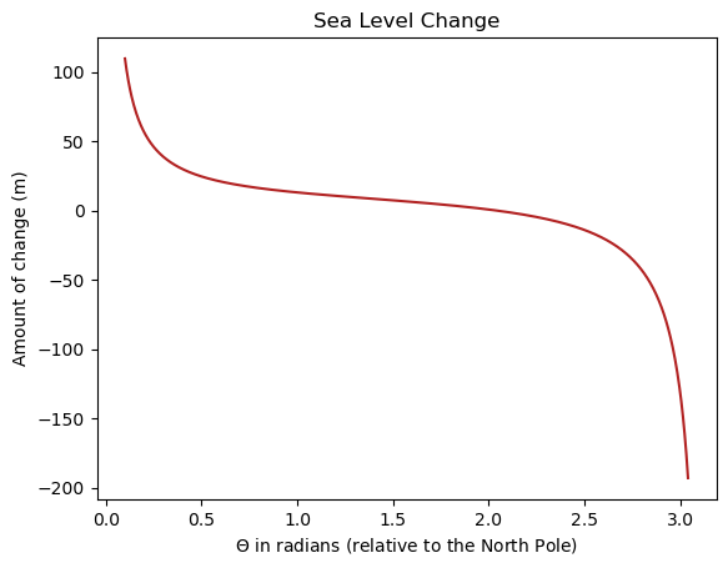
\includegraphics[width=0.6\textwidth]{images/Sample graph.png}
\caption{A graph of something.}
\label{fig:random line}
\end{figure}

\section{Methodology}
This section has a subsection.
\subsection{Subsection}
This subsection contains \autoref{eq:1}.
\begin{equation}
\label{eq:1}
    h(r) = \cfrac{Q}{2\pi T} ln(\cfrac{r_i}{r_0})+h_0
\end{equation}

\section{Results}

\section{Discussion}


\newpage
\addcontentsline{toc}{section}{References}
\bibliographystyle{apalike}
\bibliography{ref}

\newpage
\appendix
\section{Additional graphs and data}

\end{document}






%All other official TU Delft colours
\definecolor{donkerblauw}{RGB}{12, 35, 64}
\definecolor{turkoois}{RGB}{0, 184, 200}
\definecolor{blauw}{RGB}{0, 118, 194}
\definecolor{paars}{RGB}{111, 29, 119}
\definecolor{roze}{RGB}{239, 96, 163}
\definecolor{framboos}{RGB}{165, 0, 52}
\definecolor{rood}{RGB}{224, 60, 49}
\definecolor{oranje}{RGB}{237, 104, 66}
\definecolor{geel}{RGB}{255, 184, 28}
\definecolor{lichtgroen}{RGB}{108, 194, 74}
\definecolor{donkergroen}{RGB}{0, 155, 119}
%You can use these to change the hyperlink colour or the colour of the header or whatever. Glück Auf!